\section{基本中心化路由协议}
\subsection{协议概述} % (fold)
	\label{sub:协议概述}
		中心化路由协议是一个基于链路状态的网络层路由协议,使用的是Dijkstra算法,该协议中定义了一个服务器,负责接收区域内运行该协议的路由器的链路信息并且根据这些信息计算出整个区域内路由器的最短路径树,构造出每个路由器的转发表,并发送给对应路由器。并且在服务器中能够获取指定路由器对的最短路径。
	% subsection 协议概述 (end)
	\subsection{算法} % (fold)
	\label{sub:算法}

	% subsection 算法 (end)
	\subsection{协议特性} % (fold)
	\label{sub:协议特性}
		\subsubsection{协议流程} % (fold)
		\label{ssub:协议流程}
			\begin{enumerate}
				\item 路由器加入某个区域后,向邻居发送hello报文,并将定期发送hello报文。
				\item 路由器定期向服务器发送LS报文,服务器接收后计算对应信息并定时向路由器发送转发表。
				\item 服务器和路由器都有失效机制,当应当发送信息的路由器在一段时间没有发送信息后将其置为失效。
			\end{enumerate}
		% subsubsection 协议流程 (end)
	% subsection 协议特性 (end)
	\subsection{报文格式} % (fold)
	\label{sub:报文格式}
		基本Centralized协议中包含的报文格式有hello报文、LS报文、转发表报文三种报文格式。
		\par LS 报文:
		\begin{table}[H]
		\centering
			\begin{tabular}{|c|}
				\hline
				Command \\
				\hline
				Source address \\
				\hline
				Destination address \\
				\hline
				Metric \\
				\hline
				Repeat of last 8 bytes \\
				\hline
				$\cdots$ \\
				\hline
			\end{tabular}		
		\end{table}
		\par Forward Table 报文:
		\begin{table}[H]
		\centering
			\begin{tabular}{|c|}
				\hline
				Command \\
				\hline
				Destination address \\
				\hline
				nextHop \\
				\hline
				Repeat of last 12 bytes \\
				\hline
				$\cdots$ \\
				\hline
			\end{tabular}		
		\end{table}
		\par Hello 报文:
		\begin{table}[H]
		\centering
			\begin{tabular}{|c|}
				\hline
				Command        \\
				\hline
				Source address \\
				\hline
				Metric         \\
				\hline
			\end{tabular}
		\end{table}
		\par 普通报文:
		\begin{table}[H]
		\centering
			\begin{tabular}{|c|}
				\hline
				Command \\
				\hline
				source address \\
				\hline
				destination address \\
				\hline
				payload \\
				\hline
			\end{tabular}		
		\end{table}
		\par 报文项解释:
		\begin{enumerate}
			\item Command(1 Byte):指明这条报文的类型。
				\begin{enumerate}[]
					\item 0: 普通报文
					\item 1:hello
					\item 2:LS
					\item 3:转发表
				\end{enumerate}
			\item Source address(6 Bytes):指明发送方的源地址和监听端口。
			\item Destination address(6 Bytes):指明目的地的源地址和监听端口。
			\item nextHop(6 Bytes):下一跳IP地址和监听端口。
			\item Metric(2 Bytes):代价度量。
		\end{enumerate}
			
	% subsection 报文格式 (end)
	\subsection{协议扩展} % (fold)
	\label{sub:协议扩展}
		查找路径功能。在服务器中,实现了指定路由器对查找两者之间的最短路径的功能。
	% subsection 协议扩展 (end)
	\subsection{协议实现} % (fold)
	\label{sub:协议实现}
		\begin{enumerate}
			\item 客户端程序使用python编写,主要使用的是socket、threading等库。
			\item 使用Twisted异步编程框架编写服务器端。使用Twisted框架编写的服务器端具有低功耗、资源利用率高的特点,同时事件驱动的内在逻辑也符合该服务器的功能特性。
		\end{enumerate}
	% subsection 协议实现 (end)
	\subsection{结果} % (fold)
	\label{sub:结果}
		测试结果如下图\ref{fig:CentralizedTest1}和\ref{fig:CentralizedTest2}所示:
		\begin{figure}[H]
			\centering
			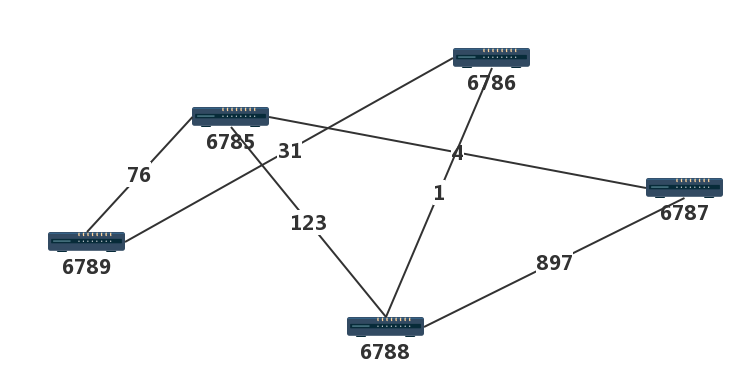
\includegraphics[scale=0.4]{imgs/topo3/tpop1.png}
			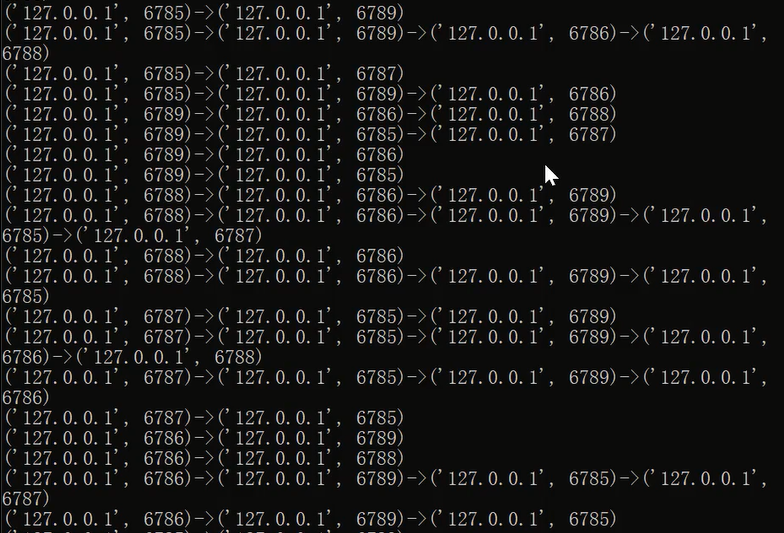
\includegraphics[scale=1]{imgs/cenTest1.PNG}
			\caption{中心化路由测试样例一}
			\label{fig:CentralizedTest1}
		\end{figure}
		\begin{figure}[H]
			\centering
			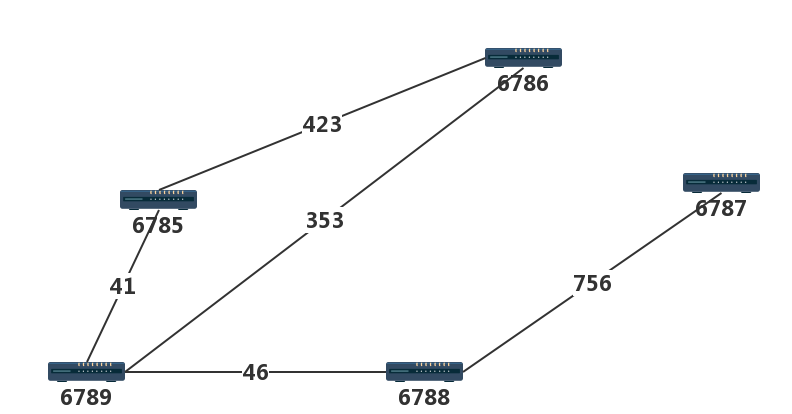
\includegraphics[scale=0.4]{imgs/topo3/topo2.png}
			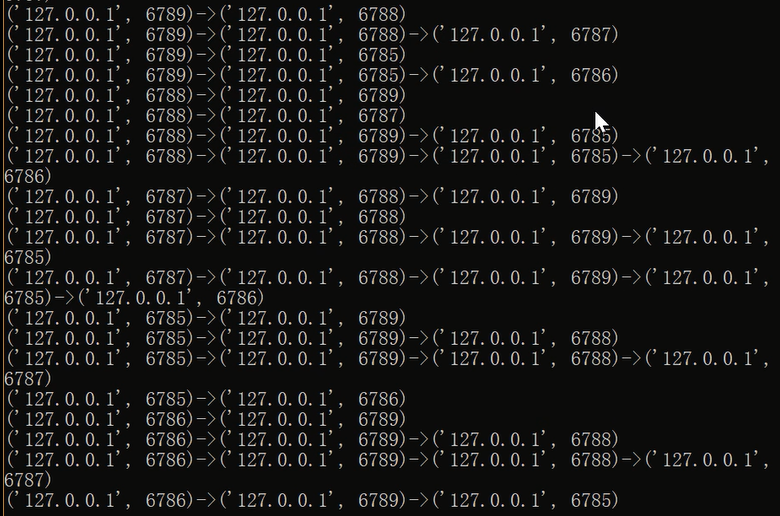
\includegraphics[scale=1]{imgs/cenTest2.PNG}
			\caption{中心化路由测试样例二}
			\label{fig:CentralizedTest2}
		\end{figure}
		成功找出了全部最短路径。
	% subsection 结果 (end)
	\subsection{总结} % (fold)
	\label{sub:总结}
		\begin{enumerate}
			\item 由于在中心化路由协议中每个路由器的转发表都是由服务器计算并且同时几乎获得,即转发表基于同一张图结构,则不存在路由循环、路由震荡等问题。
		\end{enumerate}
	% subsection 总结 (end)
% section Centralized (end)